\chapter{Planul aplicației}
\section{Introducere}
\par \textbf{În acest capitol, în secțiunea 4.2, se stabilesc funcțiile sistemului. În secțiunea 4.3 se identifică numitorul comun al funcțiilor sistemului ca fiind facilitarea funcției de \textsf{comunicare} și se  enumeră metodele prin care comunicarea la distanță se poate implementă. După analiza punctelor slabe și a punctelor forte ale acestor metode se afirmă alegerea metodei \textsf{CLIENT-SERVER} ca fiind decizia de design de urmat și implementat. În secțiunea 4.4 se proiectează un test ca suport pentru argumentarea deciziei de design (din secțiunea 4.5).}

\section{Funcțiile sistemului}

\subsection{Minimul de funcționalitate \\ de cercetat și implementat}
\par Prin analiza funcțională, bazata pe observație liberă a câtorva dintre mediile 3D existente și accesibile pe internet, am putut determina  o parte din funcțiile absolut necesare ale sistemului.
\par Aceste funcții sunt parte integrantă a cerințelor sistemului. La acestea se mai adaugă cerințele de ordin general precum: implementarea unei interfețe grafice ușor de folosit, mentenabilitatea și extensivitatea sistemului, etc.. \\
\par \textbf{Funcții ale sistemului:}
\begin{itemize}
\item Utilizatorii sistemului sunt conștienți de prezența altor utilizatori (persoane reale) în lumea virtuală. Sistemul îndeplinește funcția de liant prin facilitarea schimbului de idei între utiliztori.
\item Utilizatorii pot interacționa cu o parte dintre obiectele din umea virtuală. În unele situații, rezultatul acestei interacțiuni conduce la modificări permanente în reprezentarea lumii virtuale simulate. Sistemul îndeplinește funcția de stocare a modelului tridimensional al lumii viruale, inclusiv a starii acestui model, stare ce poate fi modificată de către utilizatori.
\item Sistemul va stoca informațiile referitoare la identificarea utilizatorilor. Această identificare nu presupune stabilirea identității persoanei reale ci are funcția de a servi ca identificator pentru un catalog al progresului utilizatorului în procesul de învățare.
\item Utilizatorii vor putea contribui la extinderea lumii virtuale prin publicarea de materiale educative dezvoltate de cătrea aceștia. Sistemul va permite contribuția utilizatorilor va avea funcția de stocare și prezentare a noilor materiale educative.
\end{itemize}

\par Cea mai mare parte dintre aceste funcții se vor implementa în aplicația software demonstrativă atașată acestui proiect.

\subsection{Funcționalitate extinsă}

\par Următoarele funcții nu vor fi incluse in software-ul demonstrtiv, dar sunt recunoscute ca necesare pentru orice sistem de învățare.

\begin{itemize}
\item Funcția de asigurare a accesibilității pentru persoanele cu deficiențe de vedere sau deficiențe motorii.
\item Funcția de redare a tuturor formelor de conținut media. Din motive tehnice și pentru complexității aplicației demonstrative, în mare măsură se vor exclude conținuturile media video și audio.
\end{itemize}

\section{Decizie privind design-ul sistemului}

\par Toate funcțiile primare ale sistemului fac referire la facilitarea comunicării între utiliztori pentru asigurarea schimbului liber de informații, sau între sistem și utilizatori cu scopul stocării și/sau accesării de date cu pentru diverse scopuri legate de funcționarea sistemului sau menținerea unui catalog al progresului utilizatorilor. Aceste schimburi de date se fac la distanță, pentru a nu condiționa geografic participarea la procesul de învățare.
\par Pentru implementarea comunicării în rețea se va alege unul dintre cele două modele general utilizate în practică: modelul client-server \ref{fig:imag5} și modelul p2p (point to point) \ref{fig:imag4}.

\par \textbf{Modelul P2P} este un model descentralizat în care fiecare nod este atât client cât și server pentru celelalte noduri din rețea. Modelul este mai dificil de implementat, consistența datelor în rețea este mai greu de menținut și administrarea este destul de dificilă. Deși modelul este mai robust prin faptul că piederea unui nod din rețea nu conduce la sistarea serviciului deoarece funcția de server este preluată de restul nodurilor; acest model nu este cel mai bun pentru implementarea unei lumi virtuale, unde consistența datelor este foarte importantă. Aceasta consistență a datelor permite tuturor utilizatorilor să perceapă aceeași lume virtuală. 

\begin{figure}[h]
    \centering
    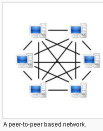
\includegraphics[]{p2p_2}
    \caption{Modelul P2P}
    \label{fig:imag4}
\end{figure}

\textbf{Modelul Client-Server} este un model centralizat în care fiecare nod client comunică și depinde de serviciile nodului server. Acest model este relativ ușor de implementat, ușor de administrat, consistența datelor poate fi verificată și inpusă la nivelul serverului și stocarea datelor poate fi facută centralizat la același nivel. Cel mai mare dezavantaj al acestui model este faptul că, pierderea accesului la server prin oprirea acestuia face tot sistemul inoperabil. Acest model este mult mai portivit pentru implementarea unei lumi virtuale și a unui mediu de învățare 3D. 

\begin{figure}[h]
    \centering
    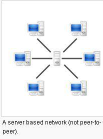
\includegraphics[]{serverbased_2}
    \caption{Modelul Client-Server}
    \label{fig:imag5}
\end{figure}

\section{Teste}
\par Testul constă în simularea comunicării dinspre server către client. Un server va incerca să timită mesaje către un număr de 20 aplicații client care salveaza în câte un fișier mesajele primite de la server. Mesajele vor avea o lungime cuprinsă între 10 și 1024 caractere.
\par Se consideră testul reușit dacă toate mesajele ajung la toate aplicațiile client în aceeași ordine și într-un timp copmarabil (sub 1 secundă distanță).
\par Pentru rularea testului se codifică două aplicații demonstrative.

\section{Argumentarea deciziei \\ pe baza rezultatelor testării}

\par Testul a fost executat cu succes. Datele obținute se află în ANEXA A.
\par Deoarece comunicarea între aplicațiile client și server sunt livrate consistent și la timp, se concluzionează faptul că se poate folosi schema client-server pentu implementarea aplicației.
